\chapter{Implementácia}
\phantomsection
V nasledujúcej kapitole budú opísané použité technológie na implementáciu práce, rozobraté dôležité časti a princíp ich fungovania, ako aj konfiguračné súbory zodpovedné za nájdenie a nápravu nedostatkov. Vo výpisoch kódu ako aj zdrojových súboroch (komentároch) sa môžu objaviť pasáže písane v anglickom jazyku. Napriek faktu, že je celá práca písaná v slovenčine, tak pre zdrojové súbory programu je angličtina vhodnejšia z hľadiska univerzálnosti a tiež kvôli predpokladanému budúcemu využitiu programu ďalšími osobami, keďže program bude verejne dostupný. Výpisy kódu v nasledujúcich kapitolách sú skrátené a iba ilustračné.

\section{Použité technológie}
 \subsection{Python}
 Python \cite{B4mfUgNUpPnXbiEr} je objektovo orientovaný, interpretovaný programovací jazyk vytvorený holanďanom Guidom van Rossom. Radí sa k~vysokoúrovňovým programovacím jazykom a umožňuje automatickú správu pamäte, teda programátor nie je nútený explicitne potrebnú pamäť alokovať a uvoľňovať Jeho výhodou je práve fakt, že je interpretovaný a teda programy napísané v~ňom nemusia byť preložené pre danú platformu, ale postačuje spustenie zdrojového kódu pomocou interpretu nainštalovaného na danom systéme. Interpret jazyka Python je dostupný pre Microsoft Windows, GNU/Linux, macOS a mnoho ďalších vstavaných a exotickejších systémov. Syntax jazyku Python je založená na syntaxi jazyku C, no zdrojový kód je čitateľnejší a na vymedzenie funkčných blokov využíva odsadenie, vďaka čomu je kód čitateľnejší. V~súčasnosti sa využíva syntax a interpret dvoch verzií, a to verzie 2.x a 3.x, ktoré sú vzájomne nekompatibilné, z~dôvodu rozdielnych syntaktických konštrukcií. Prvá zo zmienených verzií však čoskoro prestane byť podporovaná. Z~tohto dôvodu je vhodnejšie použiť na novo vyvíjané programy verziu 3.x. 
  
 Práve pre vyššie zmienené výhody, a to najmä dobrú čitateľnosť kódu, rozšíriteľnosť  medzi programátormi, ako aj spustenie na rôznych platformách bol Python zvolený za programovací jazyk pre túto diplomovú prácu.
 \subsection{YAML}
 YAML \cite{Jd4UTaVyTULvXDoN} je jazyk na serializáciu dát vo forme veľmi dobre čitateľnej pre človeka. Bol inšpirovaný konceptami a syntaxou jazykov C a Python. Dovoľuje definovať primitíva z~týchto programovacích jazykov ako zoznamy, asociatívne polia, reťazce a zároveň v~jednom súbore dovoľuje definovať viac dokumentov.
 
 Pre konfiguračné súbory na túto diplomovú prácu boli spočiatku uvažované tri metódy. Prvou možnosťou na serializáciu dát bol jazyk XML, tento formát však nie je tak dobre čitateľný pre človeka a je tu väčšia pravdepodobnosť zanesenia chýb z~dôvodu nutnosti uzatvárať značky. Druhou možnosťou bolo využitie syntaxe jazyka JSON, no problémom je, že nepodporuje vkladanie komentárov, preto nie je vhodný na konfiguračné súbory, ale skôr na strojovú serializáciu. Poslednou možnosťou bolo vytvorenie vlastnej syntaxe a vlastného analyzátoru, to je však pre potreby diplomovej práce zbytočné a hotové riešenie v~podobe YAML je dostatočné a eliminuje všetky nedostatky vyššie zmienených jazykov určených na serializáciu dát. Použitý jazyk Python naviac disponuje viacerými knižnicami na prácu s~jazykom YAML.  
 \subsection{Regulárne výrazy}
 Regulárnym výrazom sa rozumie sekvencia znakov, ktorá definuje určitý vzor \cite{sBBUt3Q3bPUfAMue}. Regulárne výrazy sa používajú na vyhľadávanie alebo výmenu reťazcov v~texte pričom na to využívajú znaky s~vopred definovanou sémantikou. V~diplomovej práci budú použité na vyhľadávanie prítomnosti alebo absencii nastavení v~konfigurácií zariadení. 

\section{Konfiguračné súbory}
Konfiguračné súbory YAML sú neoddeliteľnou súčasťou samotného programu a slúžia súbežne na viacero funkcionalít programu. Prvým z nich je \mbox{\texttt{device\_info.yaml} \ref{yaml:device_info}}, ktorý obsahuje základné údaje o testovanom zariadení, pričom pre každé testované zariadenie je separátny súbor. Druhým typom je súbor uchovávajúci informácie o module, obsahujúci regulárne výrazy na hľadanie v nastaveniach zariadenia, informácie na zjednanie nápravy a mnohé ďalšie režijné informácie. Vo výpise kódu \ref{yaml:module} je modul \texttt{01\_02\_aaa\_server.yaml} zodpovedný za definovanie AAA serveru. Ďalším YAML súborom v poradí je \mbox{\texttt{modules\_by\_facility\_layer.yaml} \ref{yaml:faclayer}}, definujúci, ktoré moduly budú spustené na zariadení podľa vrstvy hierarchického modelu, na ktorom zariadenie operuje. Posledný dôležitý YAML súbor -- \texttt{own\_variables.yaml} \ref{yaml:variables} obsahuje potrebné premenné na prípadnú zjednávanú nápravu pre danú topológiu. Podrobne budú jednotlivé súbory a ich dôležité položky rozpísané v nasledujúcich podkapitolách.
\subsection{Ukladanie informácií o zariadení}
\label{device_info}
Veľmi dôležitou súčasťou analýzy je zistenie informácií o zariadení. Na uchovanie týchto informácii slúži súbor \texttt{device\_info.yaml} \ref{yaml:device_info}. Okrem základých informácií ako mena zariadenia (\texttt{hostname}), mena súboru s exportovaným nastavením zariadenia (\texttt{config}) a verzie operačného systému (\texttt{version}) obsahuje aj ďalšie informácie. Pre správnu analýzu je nutné vedieť, či je na zariadení podpora pre IPv4 a IPv6 (\texttt{l3\_protocols}) a či sú oba protokoly povolené. Premenné \texttt{vendor} a \texttt{os} zasa určujú, o akého výrobcu sa jedná a aký operačný systém beží na zariadení. Toto sú kľúčové položky, nakoľko ich kombinácia určuje cestu ku všetkým YAML šablóna pre daného výrobcu a operačný systém. Tieto položky sa vyplňujú na základe argumentov pri spúšťaní prvotného príkazu: \texttt{netsec.py analyze ---workspace <workspace> ---vendor <vendor> ---os <os>}. Položky \texttt{facility} a \texttt{facility\_layer} sa generujú automaticky na základe analýzy exportovanej konfigurácie zariadenia. Druhá zmienená položka je podrobne rozobraná v kapitole \ref{automatic_faclayer}. Dvojica premenných \texttt{include\_modules} a \texttt{exclude\_modules} umožňujú pridávať alebo odoberať spúšťané moduly, ktoré by boli spustené na základe definície v súbore \texttt{modules\_by\_facility\_layer.yaml}, a tým personalizovať skenovanie na špecifiká danej topológie a politike nastavení pre danú firmu. Súčasťou informácií o zariadení je aj výčet jednotlivých rozhraní \texttt{interfaces} a pridelenie určitých nájdených stavov a funkcií, ktoré sú potrebné pri jednotlivých moduloch hľadajúcich nedostatky. Nutné je tiež vedieť, aké funkcionality \texttt{enabled\_functions} sú na zariadení spustené. Nemá totiž zmysel testovať bezpečnostné nastavenia pre EIGRP, pokiaľ EIGRP nie je na zariadení používané. Generovalo by to zbytočne falošne pozitívne oznámenia. Položka \texttt{input\_config\_hash} obsahuje SHA1 hash exportovanej konfigurácie, ku ktorej robíme analýzu. Dôležitá je nielen na prípadné spätné zistenie, ku ktorej konfigurácií analýza patrí, ale aj z dôvodu výslednej správy o nedostatkoch. Pretože ak by sme my alebo niekto iný pozmenil vstupnú exportovanú konfiguráciu zo zariadenia pre analýzu, ktorá už prebehla a máme výslednú správu, mohlo by to spôsobiť rozpor medzi nájdenými nedostatkami a stavom v pozmenenej konfigurácii. Takto máme dôkaz o tom, že niekto konfiguráciu pozmenil. Samozrejme hash novej konfigurácie sa dá priložiť do YAML súboru, takže ochrana nie je ideálna. Pokiaľ však vygenerujeme správu o analýze hneď po samotnej analýze nedostatkov a túto správu vytlačíme, prípadne uložíme na iné miesto, tak máme nesporný dôkaz o manipulácií so vstupnými údajmi. Pozmenenie vstupu sa však dá vykonať iba ak by mal záškodník prístup k pôvodným vstupom a chcel by spochybniť výsledky analýzy. Týmto záškodníkom môže byť aj samotný administrátor, ktorý by chcel podvrhnúť výsledky analýzy, to by bol ale veľmi extrémny prípad. Podobným spôsobom funguje aj posledná premenná \texttt{fix\_hash} uchovávajúca hash súboru s generovanou nápravou.  

\newpage
\begin{lstlisting}[frame=single,numbers=right,caption={Konfiguračný súbor \texttt{device\_info.yaml}, ktorý popisuje základné informácie o~jednom konkrétnom zariadení},label=yaml:device_info,basicstyle=\ttfamily\small\linespread{0.8}, keywordstyle=\color{black},language=python,breaklines=true]
---
hostname: "SW1_ACCESS"
config: "SW1_ACCESS_conf.txt" 
version: "15.4" 
l3_protocols:
	- "ipv4"
	- "ipv6"
vendor: "cisco"
os: "ios" 
facility: "l3sw" 
facility_layer: "collapsed_distribution_access" 
exclude_modules: []
include_modules: []
interfaces:
  Port-channel1:
	- "trunk"
	- "noip"
	- "port-channel"
  Ethernet0/0:
	- "trunk"
	- "noip"
	- "channel-group1"
  ...  
enabled_functions:
	- "rip"
	- "eigrp"
input_config_hash: "2ad9b080449de7a86e88b56fb2993b7f3ba4308e"
fix_hash: ""

\end{lstlisting}

 \newpage

\subsection{Popis modulov}
\label{module}
Základným stavebným pilierom celého programu sú moduly alebo inak povedané konfiguračné súbory YAML. Obsahujú všetky dôležité náležitosti potrebné k nájdeniu doporučeného nastavenia, respektíve jeho neprítomnosti na zariadení, dáta k zjednaniu nápravy, ako aj notifikačné informácie pre správu o analýze. Všetky komentáre, ktoré sú prítomné v YAML moduloch budú zobrazené v správe o analýze.

Pomenovanie modulov, napríklad \texttt{01\_02\_aaa\_server.yaml} \ref{yaml:module} je charakteristické dvojicou čísiel. Prvá dvojica je rovnaká pre viacero modulov a identifikuje oblasť, o ktorú sa modul stará, napríklad nastavenia AAA. Druhá dvojica je unikátna vrámci oblasti AAA, pričom v ostatných oblastiach môže byť použité rovnaké číslo. Toto číslovanie je povinné, pri pridaní nového modulu do oblasti je potreba zachovať číslovanie a zároveň druhá dvojica čísiel sa nemôže v danej oblasti opakovať. Číslovanie bolo použité z dôvodu, aby sa moduly spúšťali v želanom poradí, nebolo nutné rekurzívne spúšťanie, kde bolo nutné definovať viac náväzností ako v súčasnosti. Naviac to umožňuje pri generovaní správy s nedostatkami vypisovať spolu podobné moduly z jednej oblasti.\\  


\begin{lstlisting}[frame=single,numbers=right,caption={Konfiguračný súbor \texttt{01\_02\_aaa\_server.yaml}, ktorý popisuje základné informácie o~jednom konkrétnom zariadení},label=yaml:module,basicstyle=\ttfamily\small,rulecolor=\color{black}, keywordstyle=\color{black},language=python,breaklines=true]
---
type: "m"
facility_type: []
check_if_l3_protocol: []
check_if_function: []
run_after_module: "01_01_aaa_new_model.yaml"
run_after_module_match_status: "none"
applicable_to_interface_type: []
non_applicable_to_interface_type: [] 
cannot_determine_search_or_fix: "false" 
cannot_determine_search_or_fix_comment: ""
eliminated: "false" 
name_cmd_general: "AAA server set"
name_of_area: "Authentication, Authorization, Accounting"
default_cmd_general_severity: "high" 
user_cmd_general_severity: "none"
regex_cmd:
- '^(radius|tacacs) server (.+)$(?:.*\r?\n(?!\!))+?^.*address ipv[46].+$(?:\r?\n^.*key.+$)?(?:.*\r?\n)*?(?=\!)'
- '^.*(radius|tacacs)-server host .*$(\r?\n^.*(radius|tacacs)-server key.*$)?'
- '^.*(radius-server|tacacs-server) host .* key.+$'
regex_context: ""
regex_cmd_occurrence: "occurrence"
cmd_match_status: "not run"
general_comment: ""
mark_module_as:
- NOMODULE: "none"
- 01_03_aaa_group.yaml: "matched by equivalent"
- 01_03_aaa_group.yaml: "matched by equivalent"
matched_values: []
public_vars:
- aaa_type: "group(1)"
- aaa_server_name: "regex_cmd[0].group(2)"
- aaa_ip: ""
- aaa_key: ""
secret_vars: []
eliminate_all_matched: "false"
eliminate_prefix: ""
fix_cmd: 
- '$aaa_type server $aaa_server_name'
- 'address ipv4 $aaa_ip'
- 'address ipv6 $aaa_ip'
- 'key $aaa_key'
fix_to_apply: "" 
fix_cmd_notice: ""
fix_cmd_ignore: "false"
fix_cmd_ignore_comment: ""
fix_cmd_false_positive: "false"
fix_cmd_false_positive_comment: "" 
affected_ports: []
affected_context: []
explicit_ignored_ports: []
explicit_ignored_ports_comment: "" 
\end{lstlisting}
\vspace{1em}
\noindent
Premenné a ich význam:
\begin{itemize}
	\item \texttt{type}\,--\,môže nadobudnúť štyri hodnoty, ktoré kopírujú rozdelenie príkazov z kapitoly \ref{rozdelenie_prikazov}, preto ich význam a motivácia už nebudú ďalej rozoberané.
	\item \texttt{facility\_type}\,--\,aj keď definujeme moduly, ktoré sa majú spustiť na základe príslušnosti zariadenia vo vrstve hierarchického modelu, môžu nastať situácie, kedy to nestačí. Takýmto príkladom je distribučná vrstva. Na tejto vrstve môžu byť použité buď L3 prepínače, alebo smerovače. Rozdiel je badateľný napríklad v module, ktorý overuje nastavenia natívnej VLAN trunk portov. Pokiaľ by bolo zariadenie smerovač, tak tento modul nemá zmysel spúšťať, pretože by generoval iba falošne pozitívny nález.
	\item \texttt{check\_if\_l3\_protocol}\,--\,definuje, že modul bude spustený iba ak je na zariadení povolený určitý L3 protokol napríklad IPv6. V prípade prázdnej premennej na tom aký je protokol prítomný a nastavený na zariadení nezáleží, modul bude spustený vždy.
	\item \texttt{check\_if\_function}\,--\,definované funkcie ako napríklad OSPF, ktoré musia byť prítomné na zariadení, ak má byť spustená analýza. Je to z dôvodu eliminovania falošne pozitívnych správ, pretože nemá zmysel hľadať nedostatky v OSPF, ak vôbec nie je na zariadení nastavené. V prípade prázdnej premennej, nezáleží na tom, aké funkcie sú prítomné a nastavené na zariadení, modul bude spustený vždy.
	\item \texttt{run\_after\_module}\,--\,špecifikovanie modulu, ktorý musí byť spustený pred aktuálnym. Tejto premennej nemusí byť vždy priradená hodnota.
	\item \texttt{run\_after\_module\_match\_status}\,--\,zväzujúca informácia s predchádzajúcou položkou. Pri definovaní \texttt{none} stačí ak daný predchádzajúci modul bol spustený. Ak bude hodnota \texttt{error}, príde k spusteniu aktuálneho modulu iba v prípade neúspechu predchádzajúceho modulu. Analogicky funguje hodnota \texttt{successful}, kedy musí predchádzajúci modul skončiť úspechom, aby sa aktuálny spustil.
	\item \texttt{applicable\_to\_interface\_type}\,--\,v prípade ak ide o modul, ktorý kontroluje rozhrania, teda \texttt{type: ``i``}, tak sa môže špecifikovať zoznam, na základe ktorého sa bude testovať iba prítomnosť nastavenia na rozhraní, ktoré má určité nastavenie, napríklad na prístupových portoch \texttt{access}. V prípade viac ako jednej hodnoty v tomto zozname sa použije logická funkcia OR, a prítomnosť nastavenia sa bude hľadať na všetkých rozhraniach, ktoré spĺňajú aspoň jeden z definovaných prvkov zoznamu. V prípade prázdneho zoznamu sa bude nastavenie hľadať na všetkých rozhraniach bez výnimky.
	\item \texttt{non\_applicable\_to\_interface\_type}\,--\,premenná, ktorá funguje podobne ako predchádzajúca, akurát môže bližšie špecifikovať rozhranie, teda aj napriek pozitívnemu výskytu a zhode v predchádzajúcom parametre môžu nastať kombinácie, kde analýza modulom nie je na mieste. Napríklad by rozhranie malo atribút \texttt{access} a daný modul je aplikovateľný na takéto rozhrania, tak môžeme špecifikovať, že je aplikovateľný ak je \texttt{access} a zároveň nie je \texttt{shutdown}.
	\item \texttt{cannot\_determine\_search\_or\_fix}\,--\,môže nastať prípad, že nemáme špecifikované všetky premenné v \texttt{own\_variables.yaml}, prípadne pri hľadaní nedostatkov program nebol schopný premenné vyplniť. V takomto prípade sa táto premenná označí ako \texttt{True}, čo znamená, že administrátor musí spozornieť a prečítať si komentár k tomuto nálezu programu. Taktiež môže nastať stav, že nie je možné nájsť daný kontext špecifikovaný v \texttt{regex\_context} alebo v prípade nastavenia na rozhraní, nebolo nájdené rozhranie s daným nastavením napríklad \texttt{access}, na ktorého typ modul hľadá nedostatok.
	\item \texttt{cannot\_determine\_search\_or\_fix\_comment}\,--\,dodatočný komentár k vysvetleniu nadobudnutia hodnoty \texttt{true} v predchádzajúcej premennej.
	\item \texttt{eliminated}\,--\,znižuje počet falošne pozitívnych správ, program označí premennú ako \texttt{true} v prípade, že na skenovanom zariadení nie je funkcia definovaná v \texttt{check\_if\_l3\_protocol} alebo \texttt{check\_if\_function}.
	\item \texttt{name\_cmd\_general}\,--\,názov modulu, ktorý bude vidieť v záverečnej správe.
	\item \texttt{name\_of\_area}\,--\,oblasť pod ktorú spadá daný modul, obsah premennej bude viditeľný v záverečnej správe.
	\item \texttt{default\_cmd\_general\_severity}\,--\,predvolená hodnota závažnosti nastavenia respektíve jeho nedostatku. 
	\item \texttt{user\_cmd\_general\_severity}\,--\,špecifická hodnota závažnosti nastavenia respektíve jeho nedostatku zmenená administrátorom, ktorá bola zistená analýzou rizík. 
	\item \texttt{regex\_cmd}\,--\,regulárny výraz potrebný na nájdenie nastavenia. V prípade viac ako jedného reťazca v zozname sa použije logická funkcia OR pričom pri neúspešnom hľadaní prvého výrazu sa skúša ďalší v poradí. Hľadanie sa rozumie ako úspešné, pokiaľ aspoň jeden z regulárnych výrazov nájde zhodu v konfigurácií zariadenia. Všetky regulárne výrazy sú si rovnocenné a hľadajú rovnaké nastavenie, ale s rozličnou syntaxou.
	\item \texttt{regex\_context}\,--\,kontext pod ktorým sa hľadá regulárny vyraz z \texttt{regex\_cmd}. V tejto premennej sa nachádza tiež regulárny výraz, využitá je iba v prípade bodu 4 kapitoly \ref{rozdelenie_prikazov}.
	\item \texttt{regex\_cmd\_occurrence}\,--\,nie vždy je žiadúce aby hľadaný regulárny výraz našiel zhodu, pretože niektoré nastavenia zariadení spôsobujú bezpečnostnú hrozbu. Môžu byť prednastavené už od výroby alebo aplikované administrátormi. Z tohto dôvodu táto premenná pri nadobudnutej hodnote \texttt{occurence} definuje, že hľadaný regulárny výraz musí nájsť dané nastavenie a musí byť v zariadení prítomné. Naopak \texttt{non-occurence} znamená, že analýza modulom je úspešná, ak daný regulárny výraz nenájde žiadnu zhodu. 
	\item \texttt{cmd\_match\_status}\,--\,definuje úspešnosť \texttt{successful} alebo neúspešnosť \texttt{error} pri hľadaní regulárneho výrazu. Taktiež zo začiatku ešte nespustený modul označuje ako \texttt{not run}. V prípade, že existuje ešte nejaký modul, ktorého nastavenie implikuje súčasný modul, tak sa v tejto premennej ocitne reťazec \texttt{matched by equivalent}.
	\item \texttt{mark\_module\_as}\,--\,ako už bolo spomenuté v predchádzajúcom bode, tak pri úspešnom nájdení nastavenia respektíve pri explicitne vyžiadanej neprítomnosti nastavenia môžeme označiť iný modul povolenými hodnotami z predchádzajúceho bodu. Poradie v zozname je ekvivalentné  s poradím z premennej \texttt{regex\_cmd}. V prípade príkladu z výpisu nižšie to znamená, že pri úspešnom nájdení prvého regulárneho výrazu sa neoznačí žiaden modul. Pokiaľ sa však nenájde zhoda s prvým regulárnym výrazom testuje sa ďalší a pri jeho zhode sa označí modul \texttt{01\_03\_aaa\_group.yaml} ako \texttt{matched by equivalent}.
	\item \texttt{general\_comment}\,--\,všeobecný komentár, do ktorého sa ukladajú rôzne výstupy a upozornenia z programu.
	\item \texttt{matched\_values}\,--\,všetky zhody, ktoré sa nájdu v nastavení zariadenia budú uložené do tejto premennej. Z hľadiska anonymizácie výstupnej správy je však možné nič do tejto premennej programom nezapisovať.
	\item \texttt{public\_vars}\,--\,na zjednanie nápravy je často potrebné poznať premenné do niektorých príkazov, ktoré nastavujú zariadenie. Tie môžeme získať z úspešného nájdenia príkazu v konfigurácií, alebo zo súboru \texttt{own\_variables.yaml}. Detailnejšie sa problémom zaoberá kapitola \ref{variables_generate}.
	\item \texttt{secret\_vars}\,--\,nie je v súčasnej dobe využitá, počíta sa s premiestnením premenných na zjednanie nápravy z \texttt{public\_vars}, ktoré by sa nemali uchovávať z bezpečnostných dôvodov, napríklad rôzne heslá, ktoré sú súčasťou príkazov.
	\item \texttt{eliminate\_all\_matched}\,--\,administrátor zvolí túto hodnotu \texttt{true} ak máme \texttt{regex\_cmd\_occurrence: non-occurence}, teda ak sa nájde v nastavení príkaz, ktorý by tam nemal figurovať.
	\item \texttt{eliminate\_prefix}\,--\,súvisí z prechádzajúcou premennou a definuje reťazec, ktorý sa pridá k nájdenému nastaveniu, ktoré by sa v ideálnom prípade nemalo v konfigurácií zariadenia nachádzať a tým toto nastavenie eliminuje. Príkladom môže byť prefix \texttt{no} alebo \texttt{delete}.
	\item \texttt{fix\_cmd}\,--\,príkaz zjednávajúci nápravu. Pokiaľ má príkaz viacej riadkov, každý riadok sa píše ako zvlášť položka zoznamu. Je to z dôvodu  lepšej čitateľnosti a jednoduchšieho pridávania premenných, ktoré majú začiatočný symbol \texttt{\$}. Platí, že sa môžu použiť premenné iba definované v danom module v premennej \texttt{public\_vars}.
	\item \texttt{fix\_to\_apply}\,--\,generované programom, výsledné príkazy s vyplnenými premennými v jednom reťazci.
	\item \texttt{fix\_cmd\_notice}\,--\,Poznámka, ktorá môže byť pridaná a oznamuje prípadné problémy, ktoré by mohli vzniknúť aplikovaním nápravy.
	\item \texttt{fix\_cmd\_ignore}\,--\,administrátor môže zadať \texttt{true} pokiaľ nechce aby sa generovala náprava pre tento typ modulu.
	\item \texttt{fix\_cmd\_ignore\_comment}\,--\,komentár a zdôvodnenie, prečo administrátor nechce povoliť automatické generovanie nápravy
	\item \texttt{fix\_cmd\_false\_positive}\,--\,administrátor môže zadať \texttt{true} pokiaľ je nález falošne pozitívny.
	\item \texttt{fix\_cmd\_false\_positive\_comment}\,--\,komentár a zdôvodnenie, prečo ide o falošne pozitívny nález.
	\item \texttt{affected\_ports}\,--\,výpis rozhraní, ktoré absentujú dané nastavenie. Táto premenná je programom vyplnená iba ak \texttt{type: ``i``}.
	\item \texttt{affected\_context}\,--\,výpis kontextov, ktoré absentujú dané nastavenie. Táto premenná je programom vyplnená iba ak \texttt{type: ``c``}.
	\item \texttt{explicit\_ignored\_ports}\,--\,výpis rozhraní, ktoré sú explicitne vylúčené z analýzy.
	\item \texttt{explicit\_ignored\_ports\_comment}\,--\,komentár a zdôvodnenie, prečo boli rozhrania vylúčené.
\end{itemize}
\vspace{1em}

Zaujímavou časťou je označovanie iných modulov bez ich samotného spustenia pomocou reťazca \texttt{mark\_module\_as}. Dôležité je povedať, že takéto označovanie iných modulov je možné iba v prípade úspešnosti aktuálneho modulu. Pri nájdení chyby respektíve nedostatku to nie je možné. Iný modul je možné označiť vopred, teda ešte pred jeho samotným spustením, v tom prípade k jeho spusteniu ani nedôjde. Je však možné nejaký modul označiť aj spätne, pričom ak v označovanom module bola predtým nájdená chyba a vygenerovaná náprava, tak sa táto náprava eliminuje. Pri takomto spätnom a doprednom označovaní sa odporúča modul označiť ako \texttt{matched by equivalent}.

\newpage
\subsection{Súbor popisujúci vrstvy a moduly}
Program má ako jednu z požiadaviek minimalizovať počet falošne pozitívnych hlásení. Jeden z prístupov, ktorý má tomuto zamedziť, je spúšťanie kontroly prítomnosti nastavení  na základe umiestnenia zariadenie v hierarchickom modeli siete. Preto je nutné špecifikovať, ktoré moduly majú byť spustené na zariadeniach príslušnej vrstvy. Rozdelenie vrstiev je spomenuté v kapitole \ref{hierarchydesign} a na základe tohto rozdelenia je vytvorený aj súbor \texttt{modules\_by\_facility\_layer.yaml}. Následný výpis kódu \ref{yaml:faclayer} je len ilustračný a skrátený, kde bodky symbolizujú pokračovanie. Jeden YAML modul, môže byť definovaný na viacerých vrstvách. Špeciálnym prípadom je vrstva \texttt{all}, ktorá vlastne ani vrstvou nie je. Ide o zápis, ktorý odstraňuje redundanciu, teda moduly v nej definované by museli byť zadané povinne na každej vrstve, čo by spravilo súbor menej prehľadným a aj komplikovalo editáciu.

\begin{lstlisting}[frame=single,numbers=right,caption={Ukážka skráteného príkladu skráteného konfiguračného súboru \texttt{modules\_by\_facility\_layer.yaml}, ktorý popisuje, aké moduly môžu byť spúšťané na jednotlivých vrstvách.},label=yaml:faclayer,basicstyle=\ttfamily\small, keywordstyle=\color{black},language=python,breaklines=true]
---
all:
- "01_01_aaa_new_model.yaml"
- "01_02_aaa_server.yaml"
...
- "02_20_session_timeout.yaml"
...
- "11_02_cdp_enable.yaml"
...
core: 
..
- "14_01_filter_private_on_wan.yaml"
..
collapsed_all:
...
- "10_01_access_vlan_1.yaml"
...
collapsed_core_distribution:
...
- "10_01_access_vlan_1.yaml"
...
distribution: 
...
- "10_01_access_vlan_1.yaml"
...
collapsed_distribution_access:
...
- "10_01_access_vlan_1.yaml"
...
access: 
...
- "10_01_access_vlan_1.yaml"
...

\end{lstlisting}

\subsection{Premenné na generovanie nápravy}
\label{variables_generate}
Pre generovanie náprav je nutná znalosť nielen samotného príkazu, ktorý problém vyrieši, ale je často potreba doplniť do príkazov premenné ktoré sa môžu pre jednotlivé testované siete líšiť. Preto vznikol YAML súbor, ktorého čiastočná ukážka je vo výpise \ref{yaml:variables}. Po spustení programu \texttt{netsec.py} s argumentom \texttt{analyze} môžeme vyplniť tento YAML súbor v príslušnom workspace. Je dobré vyplniť čo najviac premenných, ideálne všetky, pretože nikdy dopredu nevieme, ktorý hľadaný nedostatok bude potrebovať nápravu a informácie práve z tohto súboru. Pri nevyplnení niektorých premenných je administrátor notifikovaný touto skutočnosťou a môže prázdne premenné doplniť alebo ignorovať túto notifikáciu. Prioritne sa však premenné neberú z \texttt{own\_variables.yaml}, ale k ich výberu dochádza až ako k poslednej možnosti. Prioritne sa berú informácie z modulov, ktorého jeden reprezentant je v kapitole \ref{module} v premennej \texttt{public\_vars}. Tieto premenné sa mohli nájsť pri úspešnom hľadaní nejakého predchádzajúceho modulu. 

Môže nastať päť situácií s hodnotou premenných v \texttt{public\_vars}. Pokiaľ je reťazec prázdny, tak sa zoberie hodnota z \texttt{own\_variables.yaml}. Pokiaľ prázdny nie je, tak pri úspešnom nájdení pomocou regulárneho výrazu je možné vytiahnuť z tejto zhody určité skupiny, príkladom je premenná \texttt{aaa\_type: ``group(1)``} vo výpise \ref{yaml:module}. Pokiaľ pred \texttt{group(1)} nie je bližšie špecifikované, ku ktorému regulárnemu výrazu z \texttt{regex\_cmd} patrí, tak táto skupina musí byť rovnaká vo všetkých regulárnych výrazoch, ktoré sú definované v \texttt{regex\_cmd}. To je aj dosiahnuté ak sa pozrieme na všetky tri regulárne výrazy v tomto výpise. Následne môže nastať prípad, kedy potrebujeme niektorú premennú vyplniť iba v prípade úspešného nájdenia jedného z regulárnych výrazov. Vtedy použijeme konštrukciu \texttt{regex\_cmd[0].group(2)}, ktorá hovorí, že skupina 2 z regulárneho výrazu bude do premennej daná iba v prípade, že zhodu našiel prvý regulárny výraz (indexovanie od nuly). Predposledná možnosť je sa odkázať na premennú z iného modulu, kde bola premenná vopred vyplnená alebo úspešne doplnená, napríklad \texttt{01\_03\_aaa\_server\_group.yaml.aaa\_server\_type}. Túto možnosť je dobré využiť pokiaľ informácia z jedného príkazu je nutná na vytvorenie nadväzujúceho doplňujúceho príkazu, ktorý je v inom module. Posledná možnosť je natvrdo vyplniť hodnotu nejakým reťazcom.

Ako bolo už spomenuté, súbor \texttt{own\_variables.yaml} obsahuje informácie pre celý jeden workspace, môže sa stať, že pre nejaké zariadenie môžeme chcieť špecifické nastavenie odlišné od definovaného v tomto súbore. Toto je možné docieliť editáciou samotného modulu v danom adresári zariadenia, ktorý vyhľadáva a napravuje nedostatok, ale je tak možné učiniť až po pustení programu s argumentom \texttt{analyze}.
%\vspace{-0.0em}
\begin{lstlisting}[frame=single,numbers=right,caption={Ukážka skráteného príkladu vyplneného konfiguračného súboru \texttt{own\_variables.yaml} definujúceho premenné potrebné na generovanie nápravy},label=yaml:variables,basicstyle=\ttfamily\small, keywordstyle=\color{black},language=python,breaklines=true]
---
aaa_type: "radius"
aaa_server_name: "CORP_RADIUS"
...
ssh_port: "2223"
...
syslog_ipv4: "10.0.0.140"
...
ospf-router-id: "1.1.1.1"
...
allowed_vlan_on_trunk: "10,20,30"
...
...
\end{lstlisting}

\begin{figure}[H]
	\begin{center}
		\vspace*{-1cm}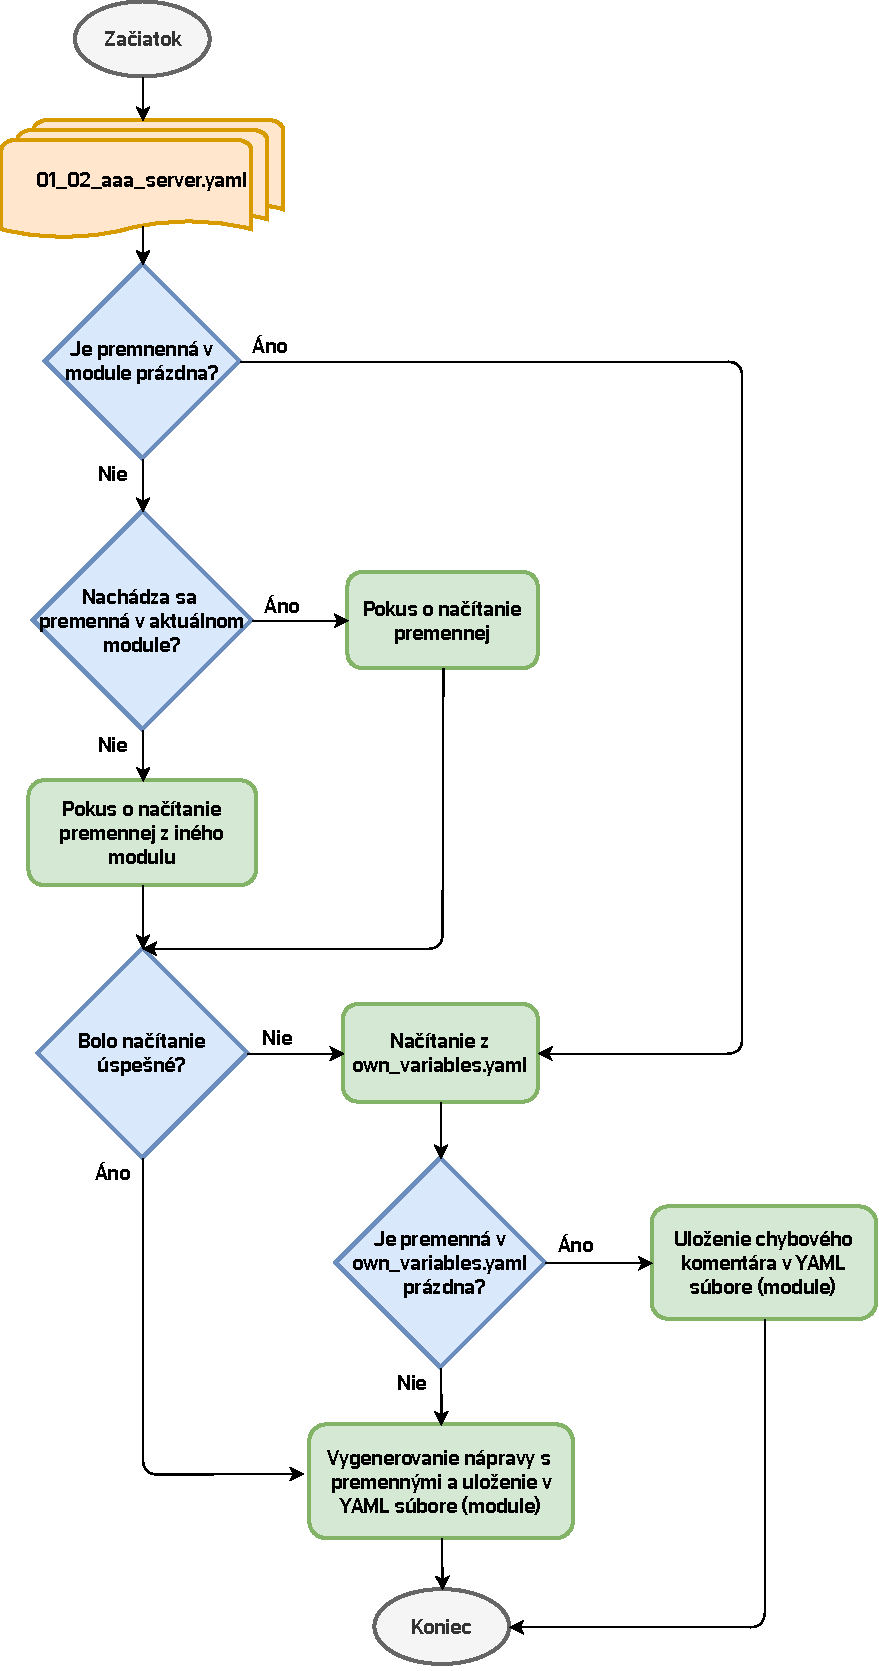
\includegraphics[scale=0.87]{obrazky/variables_fix.pdf}
	\end{center}
	\caption[Vývojový diagram opisujúci hľadanie premenných pre nápravu]{Vývojový diagram opisujúci hľadanie premenných pre nápravu}
	\label{variables_fix}
\end{figure}


\section{Popis fungovania a diagramy funkcií}
\label{popis_fungovania}
Program je vytvorený s orientáciou na budúcu možnú rozšíriteľnosť, prenositeľnosť, modularitu a udržovateľnosť kódu. Z tohto dôvodu sa nejedná o jeden skript, ktorý ma v sebe natvrdo napísané regulárne výrazy na hľadanie nedostatkov, reakciu na ne a rôzne ďalšie minoritné výstupy, ale obsahuje "moduly". Tieto moduly, viď \ref{module} sú konfiguračnými súbormi využívajúcimi syntax a sémantiku jazyka YAML a definujú správanie programu pri nájdení, odstraňovaní a notifikovaní o nedostatku na analyzovanom zariadení. Samozrejme tento koncept generuje určitú vyššiu réžiu na ukladanie nálezov, ale značne tým zvyšuje modularitu, znovupoužiteľnosť a budúcu rozšíriteľnosť.

V prechádzajúcich kapitolách a v adresárovej štruktúre opísanej v kapitole \ref{hierarchy_struct} bolo často spomenuté slovo "workspace". Jedná sa v podstate o zložku s vyexportovanými konfiguráciami, ktoré patria pod jednu sieť. Záleží od používateľa programu, ktoré všetky zariadenia považuje za jednu sieť a chce ich zanalyzovať naraz. Zároveň je však odporúčané dávať do jednej workspace zložky ideálne zariadenia operujúce na rovnakej vrstve hierarchického modelu, t.j. napríklad všetky zariadenia z danej testovanej siete, ktoré sa používajú na prístupovej (access) vrstve. Program síce obsahuje algoritmus popísaný v \ref{automatic_faclayer} na rozpoznanie zariadenia a zatriedenie do vrstvy hierarchického modelu, no jeho spoľahlivosť nie je 100\%-ná. Preto existuje prepínač, ktorý definuje, že všetky zariadenia v danej zložke (workspace) patria iba do jednej určitej vrstvy. A z tohto dôvodu je odporúčané dávať do analyzovanej zložky ideálne zariadenia operujúce na rovnakej vrstve. Je nutné taktiež podotknúť, že nie je nutné ako názov zložky používať slovo "workspace", užívateľ si tento názov môže zvoliť ľubovoľne, ide iba o demonštráciu. Pri analyzovaní siete organizácie VUT FEKT sa môže zvoliť názov zložky "sieť\_VUT\_FEKT".

\subsection{Vytvorené triedy}
Program pre svoju prácu využíva tri dôležité triedy. Prvou je abstraktná trieda \texttt{device\_info\_abstract}, z ktorej budú dediť všetky ďalšie triedy \texttt{device\_info}. Triedy \texttt{device\_info} respektíve súbor \texttt{device\_info.py} bude musieť byť vytvorený pre každého výrobcu zvlášť, pričom stačí využiť dedičnosť, podediť premenné z \texttt{device\_info\_abstract}, špecifikovať triednu premennú \texttt{vendor} a povinne implementovať metódy \texttt{fill\_variables}, \texttt{list\_interfaces}.


Druhá trieda je \texttt{device\_info} \ref{device_class} a ako už názov napovedá, tak je názov rovnaký ako YAML súbor \texttt{device\_info.yaml}. Táto trieda obsahuje metódy, v obrázku označené žltou farbou, ktoré zisťujú základné informácie o zariadení a následne ich ukladajú do inštančných premenných ilustrovaných modrou farbou v triede \texttt{device\_info\_abstract}. Niektoré metódy a všetky inštančné premenná sú zdedené z abstraktnej triedy \texttt{device\_info\_abstract}. Metódy začínajúce podtržníkmi sú pseudo privátne, metóda \texttt{\_\_init\_\_} je konštruktor a ostatné metódy sa môžu volať aj mimo tela samotnej triedy. Špeciálnym prípadom je premenná \texttt{vendor}, ktorá je triedna. Treba ju preto definovať v každom súbore \texttt{device\_info.py} u jednotlivých výrobcov zariadení. Napísanie povinných dvoch metód zmienených vyššie, ktoré sú zdedené z \texttt{device\_info\_abstract}, je nutné z dôvodu rozdielnej syntaxe jednotlivých výrobcov a operačných systémov bežiacich na zariadeniach. Je to v podstate jediné potrebné programovanie, ktoré je nutné spraviť pri rozšírení podpory programu na ďalších výrobcov. Ostatné prídavné moduly sa definujú iba pomocou konfiguračných súborov YAML, ktorého príklad je uvedený vo výpise \ref{module}.
 
Ukladanie tohto objektu do YAML súboru je nutné z dôvodu, že samotný program sa spúšťa v štyroch fázach a je žiadúce raz získané údaje uložiť, ako ich znovu vyhľadávať vo vyexportovaných nastaveniach zariadení. V prvotnej fáze spustenia programu s argumentom \texttt{analyze} sa získané informácie uložia do YAML konfiguračného súboru \texttt{device\_info.yaml} za pomoci metód \texttt{save\_object\_to\_yaml} a následne \texttt{write\_to\_yaml}. Analogicky pri spustení programu so zvyšnými troma argumentami sa na prácu s daným zariadením využijú metódy na načítanie \texttt{read\_from\_yaml} a \texttt{load\_yaml\_to\_object}.
\begin{figure}[H]
	\begin{center}
		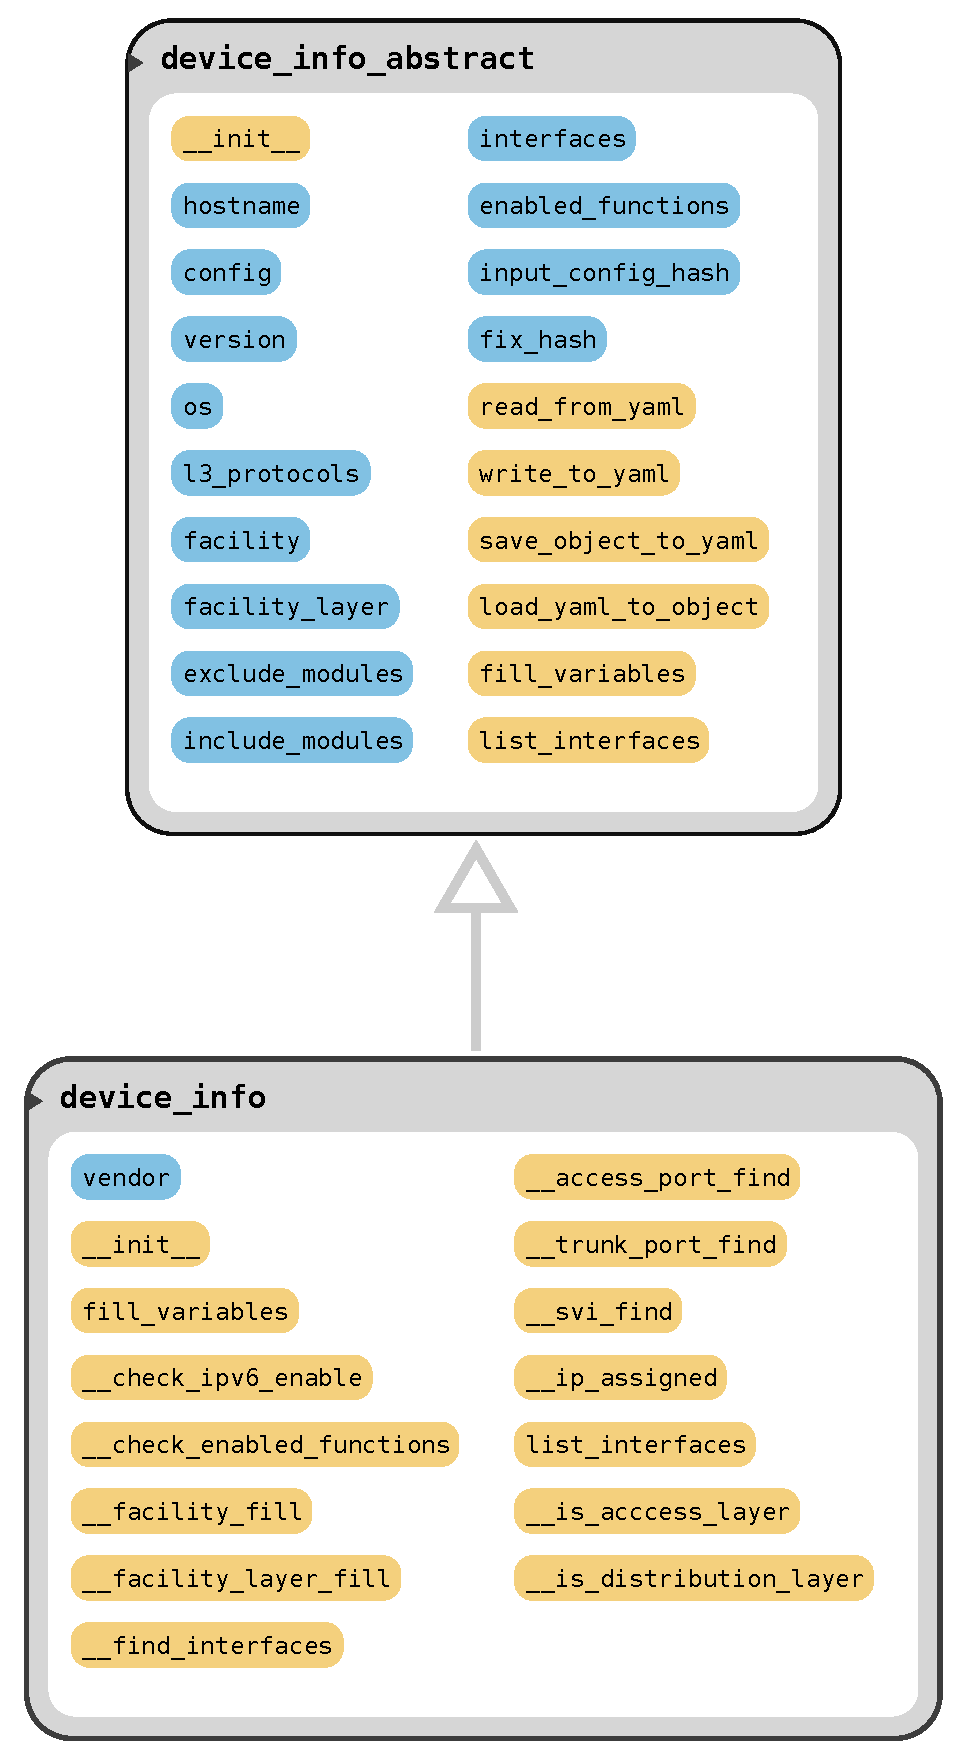
\includegraphics[scale=0.55]{obrazky/device_info_class.pdf}
	\end{center}
	\caption[Objekt \texttt{device\_info}. Inštančné/triedne premenné sú označené modrou farbou a metódy žltou farbou.]{Objekt \texttt{device\_info}. Inštančné/triedne premenné sú označené modrou farbou a metódy žltou farbou.}
	\label{device_class}
\end{figure}

Treťou triedou je \texttt{yaml\_module}, ktorá slúži na uchovanie informácií, ale aj ako zdroj informácií pri hľadaní nedostatkov a obsahuje dáta potrebné na zjednanie nápravy. Obsahuje iba štyri metódy, ktoré sú nutné pre prácu s YAML súbormi a boli popísané v predchádzajúcom odstavci. Je vidieť, že počet inštančných premenných je značne veľký, to je dané jednak generalizáciou príkazov, ktoré sieťové zariadenie konfigurujú, ale aj orientáciou a rozšírením programu do budúcnosti, kde sa ráta vyššia miera interakcie od administrátora, hlavne označovanie falošne pozitívnych nálezov, ich komentovanie a mnohé ďalšie funkcie. Tieto funkcie sú dostupné aj v súčasnosti, no komentáre sú editovateľné v YAML súbore iba pomocou textového editora. V budúcnosti sa počíta aj s vytvorením backend-u v jazyku Python a editácia vo webovom prehliadači. 
\begin{figure}[H]
	\begin{center}
		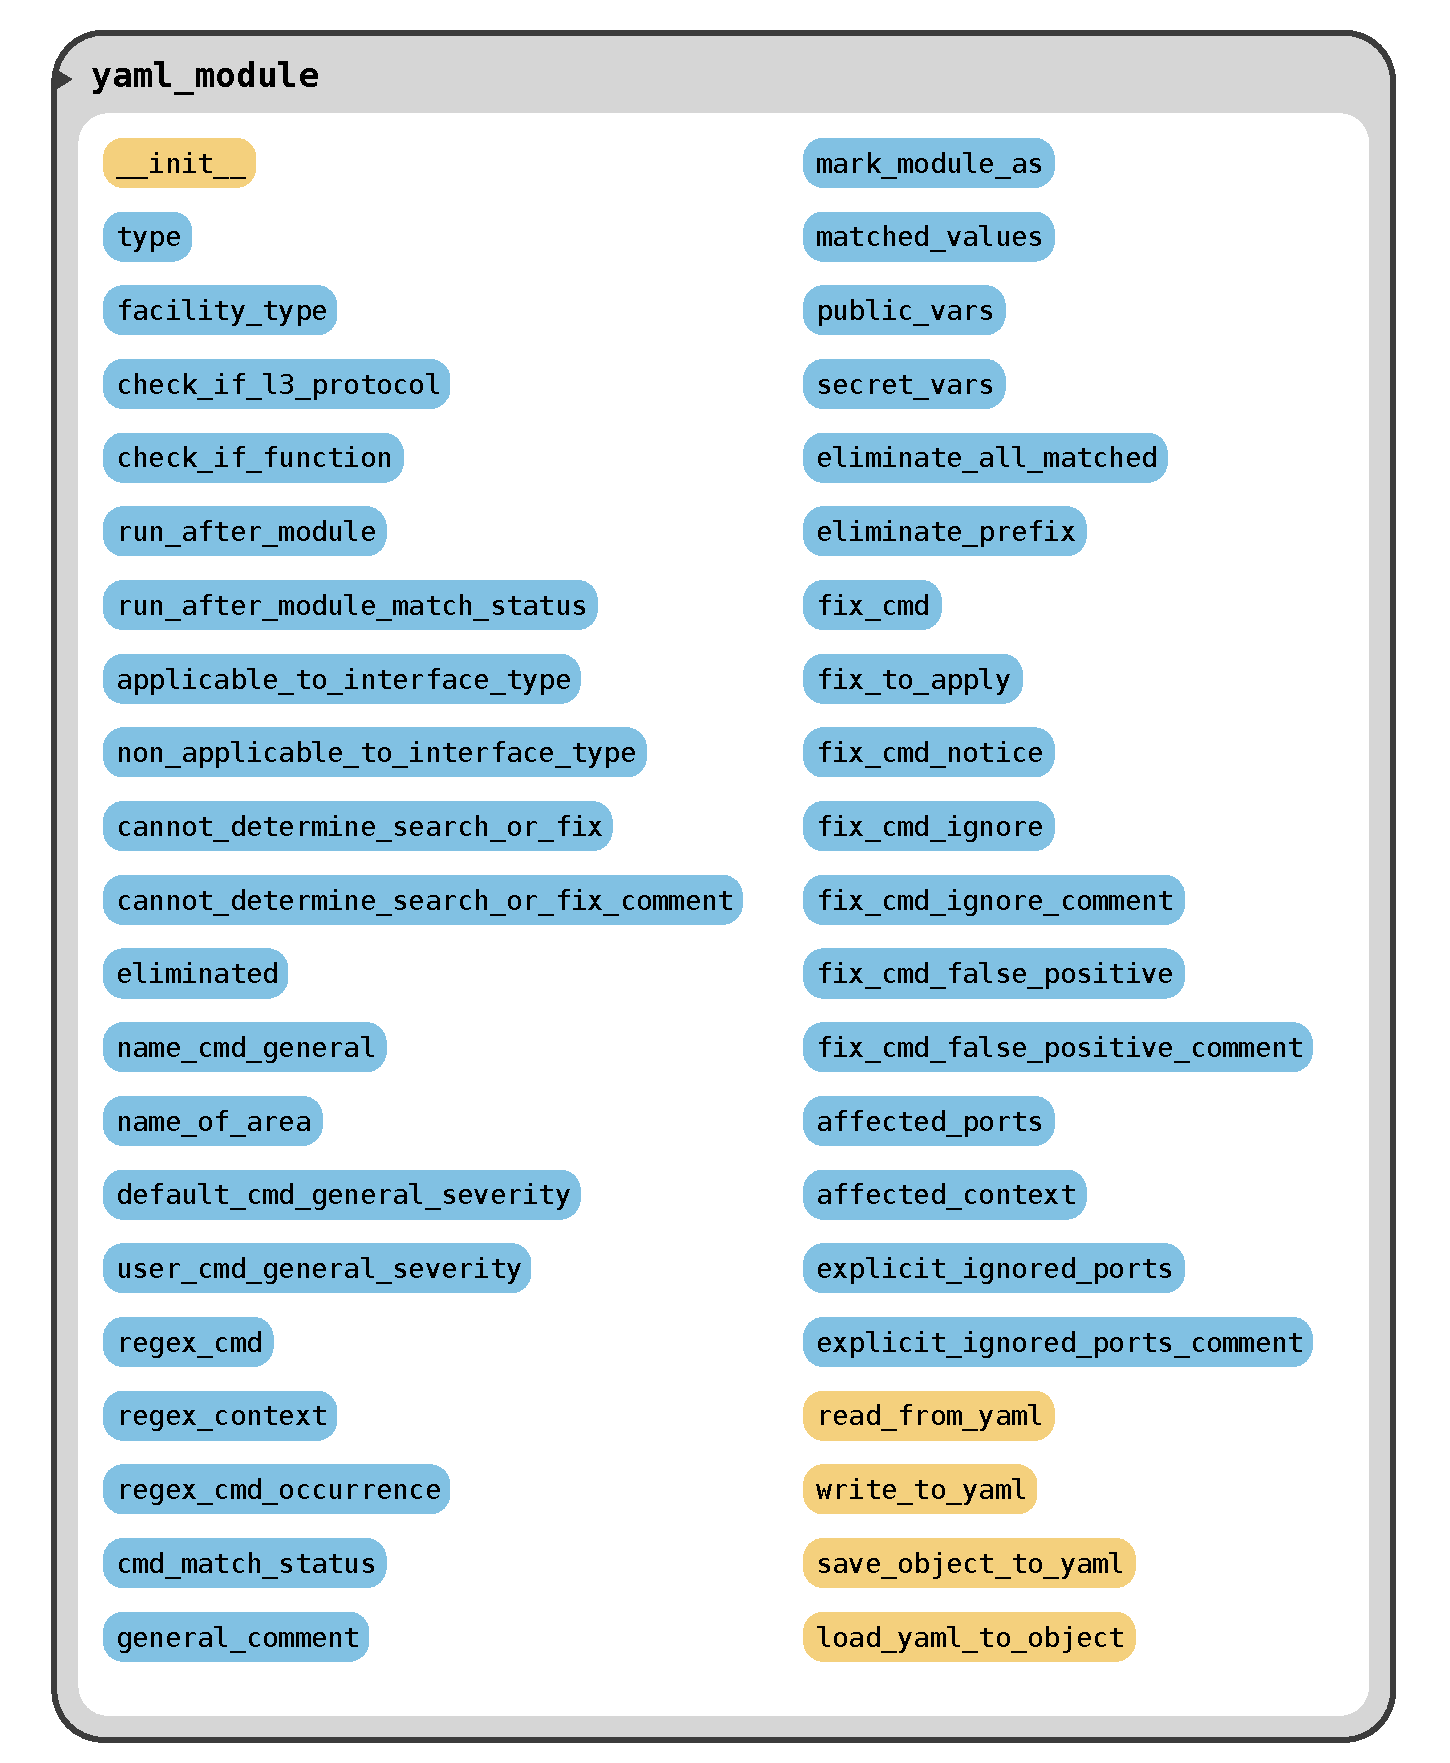
\includegraphics[scale=0.55]{obrazky/yaml_module_class.pdf}
	\end{center}
	\caption[Objekt \texttt{yaml\_module}. Inštančné/triedne premenné sú označené modrou farbou a metódy žltou farbou.]{Objekt \texttt{yaml\_module}. Inštančné/triedne premenné sú označené modrou farbou a metódy žltou farbou.}
	\label{module_class}
\end{figure}

\newpage
\subsection{Automatické zistenie vrstvy}
\label{automatic_faclayer}

Ako už bolo spomenuté viackrát, tak pre minimalizáciu falošne pozitívnych správ treba spúšťať iba tie moduly, ktoré sú nutné pre dané zariadenie na konkrétnej vrstve hierarchického modelu. Z tohto dôvodu pri spustení programu s parametrom \texttt{analyze} príde k automatickému zisteniu vrstvy hierarchického modelu, na ktorom zariadenie operuje. Algoritmus popisujúci túto činnosť \ref{fac_layer} nie je však dokonalý. Ako si môžeme všimnúť, tak pre označenie zariadenia ako ``Core`` predpokladá prítomnosť nastaveného protokolu BGP. Nie však na všetkých ``Core`` prvkoch treba mať BGP zapnuté, hlavne nie pri malých hraničných sieťach, kde sa zväčša nastavuje východzia brána. Hraničné ``Core`` zariadenia väčšinou nedisponujú mnohými nastaveniami a je veľmi obtiažne zistiť či ide naozaj o ``Core`` zariadenie. Niektoré siete zasa využívajú BGP aj ako interný smerovací protokol. Preto nie je v určitých špeciálnych prípadoch dobré sa viazať na tento vytvorený algoritmus, vo všeobecnosti však veľmi dobre funguje na rozoznanie ostatných vrstiev popísaných v kapitole \ref{hierarchydesign}.

Pri každom spustení programu s argumentom \texttt{analyze} je na konzolu zobrazená dvojica hostname zariadenia a automaticky zistená vrstva zariadenia. Teda administrátor má informáciu o tom, do akej vrstvy bolo zariadenie zaradené a prikladá informáciou o tom, kde sa dá ručne zmeniť toto rozhodnutie. 

Samozrejme je možné definovať ručne vrstvu editovaním YAML modulu pre želané zariadenia v \texttt{device\_info.yaml}. Toto však nie je úplne komfortné, a preto je možné pri prvotnom spúšťaní programu s argumentom \texttt{analyze} použiť prepínač \texttt{--facility\_layer} a definovať to pre všetky zariadenia v danom workspace. Z predchádzajúceho teda vyplýva, že je namieste separovať exportované konfigurácie zariadení podľa vrstvy do separátnych workspace a teda nepoužívať jeden workspace pre celú topológiu.  

\vspace{2em}
\noindent
Predpoklady pre rozhodnutie príslušnosti zariadenia k danej vrstve:
\begin{itemize}
	\item Core\,--\,zapnutý protokol BGP
	\item Distribution\,--\,použité dynamické IGP protokoly/použitie protokolov FHRP/ smerovatelné porty/ip adresa na portoch
	\item Access\,--\,spanning tree edge port/spanning tree BPDU guard/špecifikovaná access VLAN/802.1x/port security(maximum MAC adries na port) 
\end{itemize}

\begin{figure}[H]
	\begin{center}
		\vspace*{-1cm}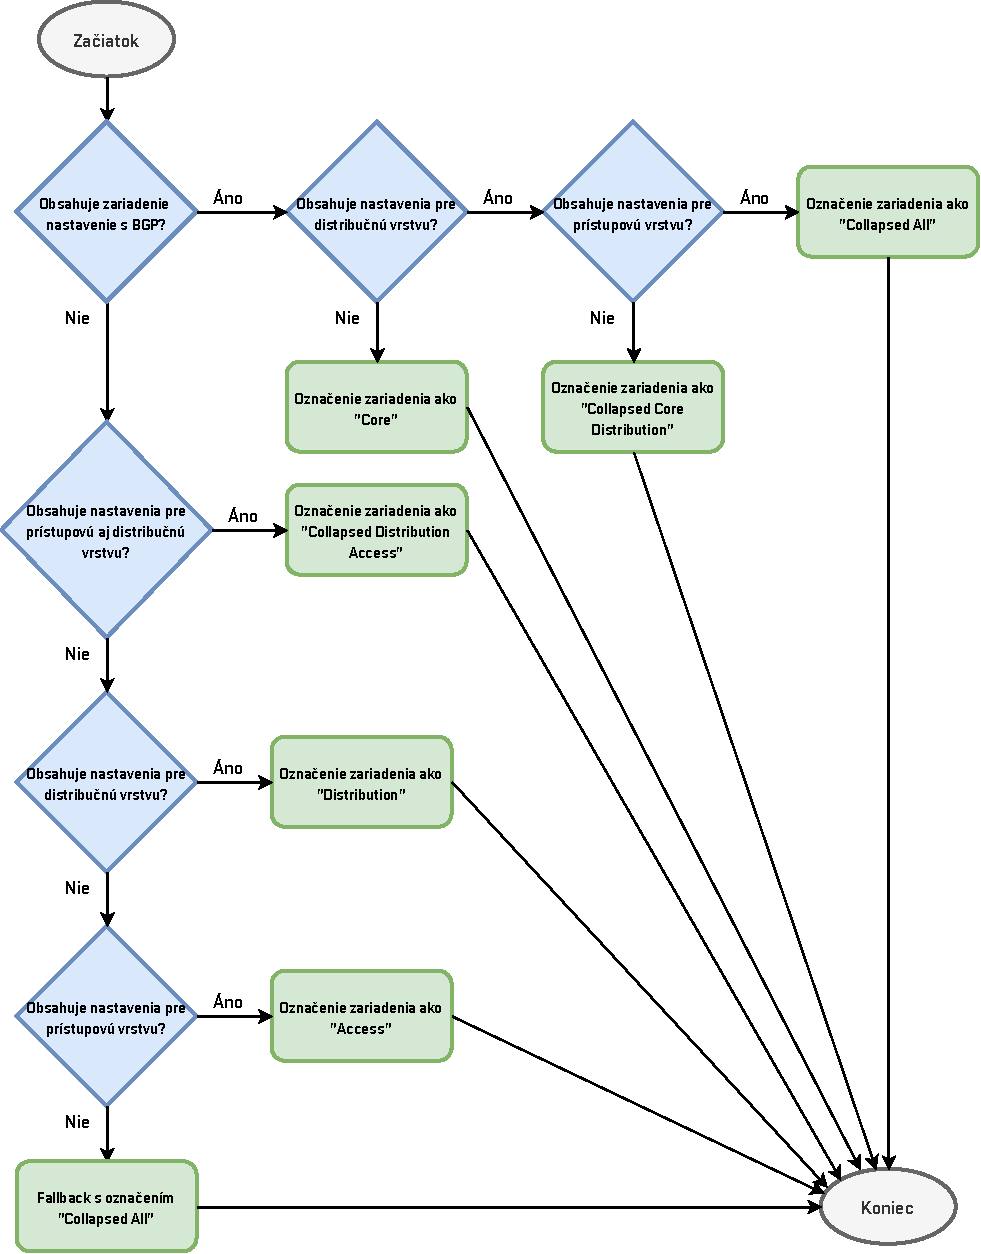
\includegraphics[scale=0.8]{obrazky/fac_layer.pdf}
	\end{center}
	\caption[Vývojový diagram opisujúci automatické zistenie vrstvy]{Vývojový diagram opisujúci automatické zistenie vrstvy}
	\label{fac_layer}
\end{figure}


\subsection{Pridávanie modulov a nových výrobcov}
V prípade rozšírenia a pridania modulu na hľadanie nedostatku pre zariadenia Cisco s IOS je potrebné:
\begin{enumerate}
	\item Definovanie regulárneho výrazu hľadajúceho nastavenie.
	\item Zatriedenie typu hľadaného príkazu podľa \ref{rozdelenie_prikazov}.
	\item Vytvorenie YAML modulu, ktorého šablóna je v zložke \texttt{examples}.
	\item Vytvorenie nutných premenných pre príkazy v súbore \texttt{own\_variables.yaml}.
	\item Pridanie YAML modulu do súboru \texttt{modules\_by\_facility\_layer.yaml} k príslušnej vrstve.
\end{enumerate}

\vspace{1em}
\noindent
V prípade rozšírenia podpory programu pre ďalšieho výrobcu je potrebné:
\begin{enumerate}
	\item Vytvorenie súborovej štruktúry \texttt{modules/výrobca/os}.
	\item Vytvorenie modulov podľa predchádzajúceho postupu. Moduly by mali odpovedať odporúčaniu z návrhu \ref{check_list}.
	\item Vytvorenie súboru \texttt{device\_info.py} dedením \texttt{device\_info\_abstract} a implementovanie nutných metód. Taktiež je potreba vytvoriť metódy na zistenie základných nastavením ktoré sú rozdielne u každého výrobcu a operačného systému, keďže majú inú syntax. Údaje, ktoré je treba zistiť, sú jednotlivé inštančné premenné súboru \texttt{device\_info\_abstract.yaml}.  
\end{enumerate}

\section{Spúšťanie programu}
Beh programu sa rozdeľuje do štyroch fáz. Je to z dôvodu, že pri naplnení niektorých súborov sa môže alebo je potrebné editovať ich obsah.


\begin{enumerate}
	\item Inicializácia\,--\,je dôležitá pre zistenie základných informácií o zariadeniach v definovanom workspace. Zistené údaje sú napríklad jeho meno, role jednotlivých rozhraní, zatriedenie zariadenia do hierarchického modelu siete, a tým zistenie, ktoré moduly sa budú spúšťať v nasledujúcej fáze. Zjednodušený postup práce programu tejto časti je znázornený pomocou vývojového diagramu \ref{netsec_analyze}.
	\item Hľadanie nedostatkov a generovanie nápravy\,--\,pre každé zariadenie je spustený zoznam modulov zodpovedajúcich vrstve, na ktorej zariadenie pracuje. Je dobré po úvodnej analýze vyplniť súbor \texttt{own\_variables.yaml}, kde sa nachádzajú premenné potrebné pre nápravu v prípade príkazov, ktoré potrebujú dodatočné informácie. Diagram \ref{netsec_audit} opisujúci hlavnú časť programu je veľmi zjednodušený, zovšeobecnený a abstraktný. V prípade záujmu je možné nahliadnuť do zdrojového súboru \texttt{netsec.py} do metód \texttt{audit\_check} a \texttt{audit\_analyze\_module}.
	\item Generovanie záverečnej správy\,--\,diagram pre túto časť programu nie je potrebný nakoľko ide o priamočiaru prácu. Otvoria sa všetky moduly v zložke každého zariadenia, zistí sa stav hľadania nedostatkov a všetky údaje sa použijú na vytvorenie záverečnej HTML správy aj so štatistickými informáciami. Príklad tejto správy je k nahliadnutiu v kapitole \ref{sprava_nedostatky}.
	\item Vyexportovanie súborov pre nápravu\,--\,pre túto časť programu nie je taktiež nutná vizualizácia, keďže sa zoberú vygenerované reťazce nápravy z každého YAML modulu v adresári pre konkrétne zariadenie a pridajú sa do textového súboru, ktorý sa následne bude aplikovať na zariadenie. Tento nápravný textový súbor je vygenerovaný pre každé zariadenie. Môže byť aplikovaný ručne pomocou nakopírovania do konzole alebo v prípade existencie automatických nasadzovacích nástrojov ako Ansible, sa táto činnosť môže spraviť automatizovane.
\end{enumerate}

\vspace{2em}
\begin{figure}[H]
	\begin{center}
		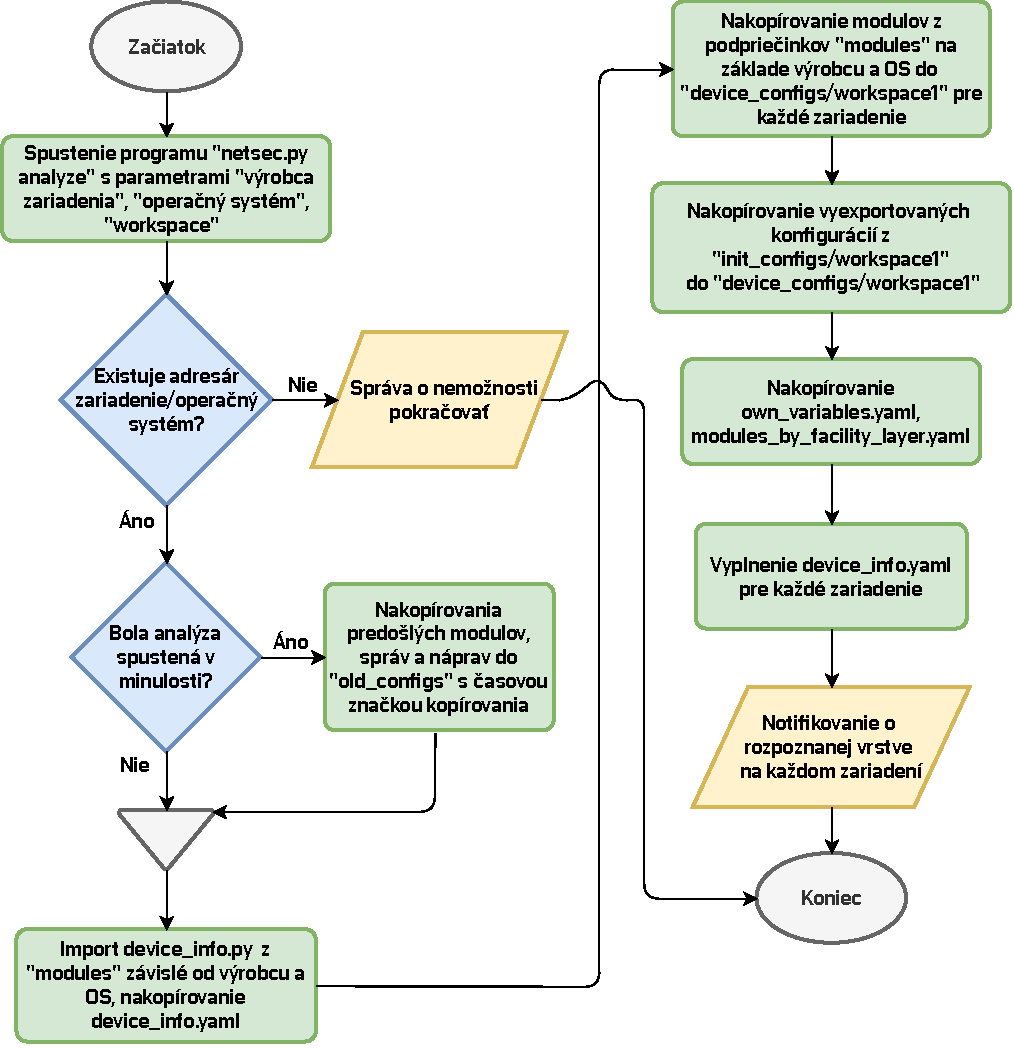
\includegraphics[scale=0.8]{obrazky/netsec_analyze.pdf}
	\end{center}
	\caption[Inicializácia programu pomocou argumentu \texttt{analyze}.]{Inicializácia programu pomocou argumentu \texttt{analyze}.}
	\label{netsec_analyze}
\end{figure}

\begin{figure}[H]
	\begin{center}
		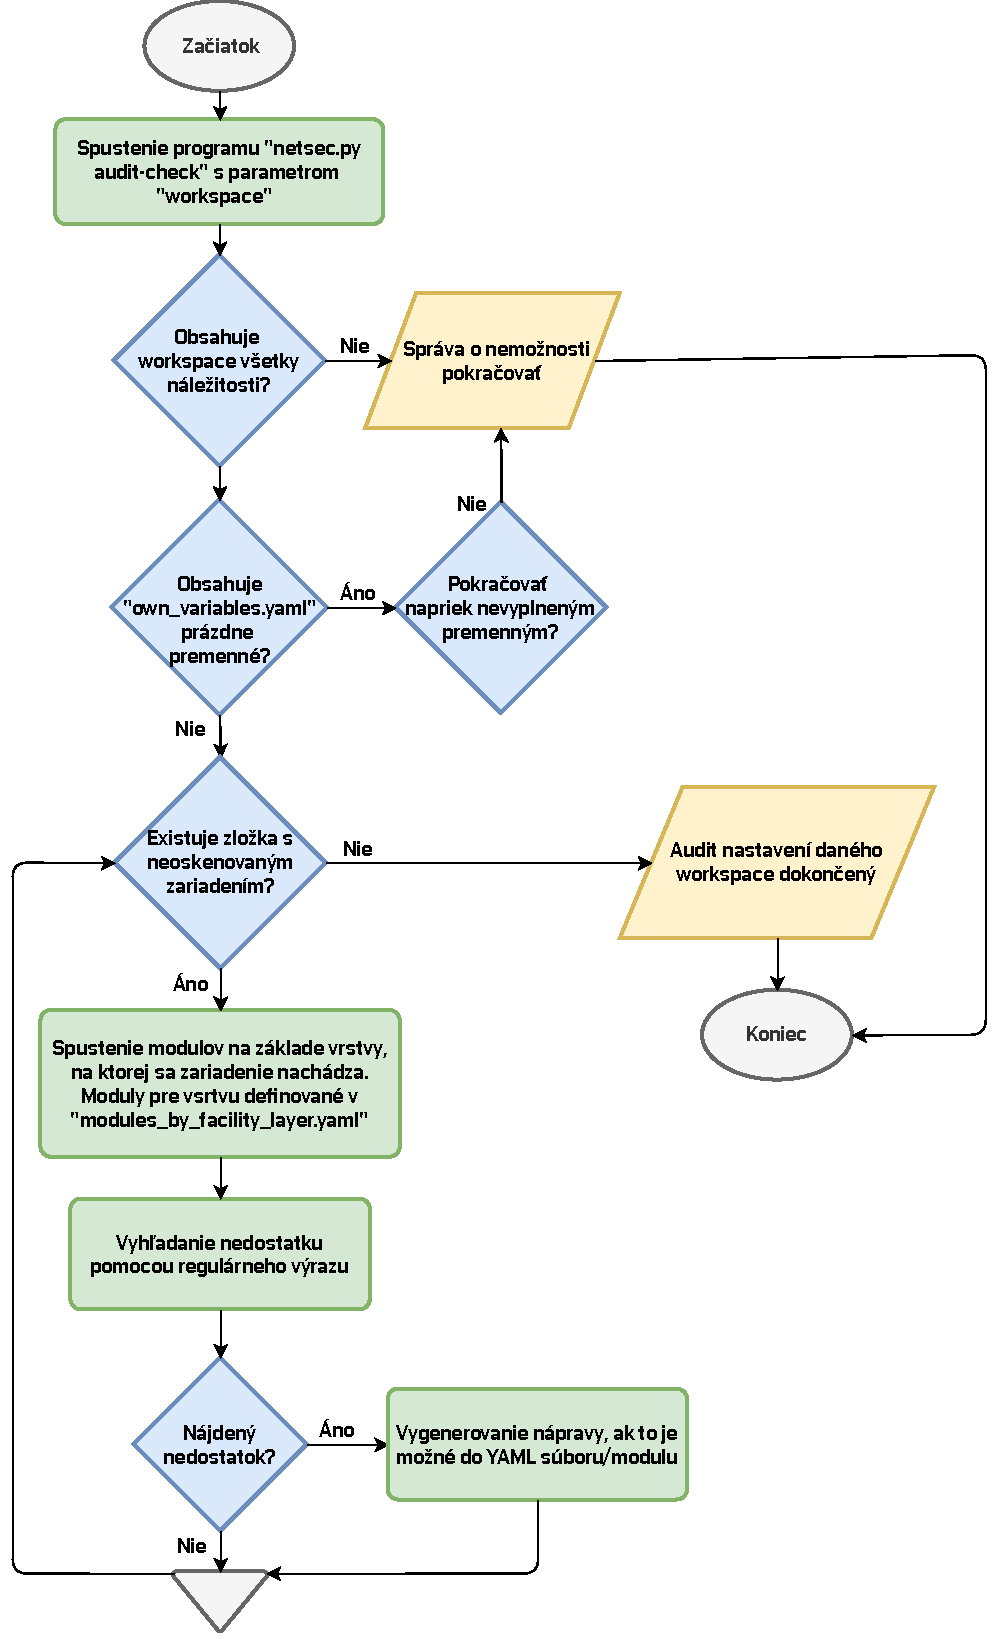
\includegraphics[scale=0.8]{obrazky/netsec_audit.pdf}
	\end{center}
	\caption[Veľmi zjednodušený pohľad na prácu hlavnej časti programu zodpovednú za nájdenie nedostatkov a vygenerovanie ich nápravy spustením pomocou argumentu \texttt{audit-check}.]{Veľmi zjednodušený pohľad na prácu hlavnej časti programu zodpovednú za nájdenie nedostatkov a vygenerovanie ich nápravy spustením pomocou argumentu \texttt{audit-check}.}
	\label{netsec_audit}
\end{figure}

\section{Správa s nedostatkami}
\label{sprava_nedostatky}
Po úspešnej analýze nastavení zariadení je možné pomocou argumentu \texttt{generate\_report} vytvoriť správu o analýze s nájdenými nedostatkami. Správa obsahuje základné informácie o zariadení zo súboru \texttt{device\_info.yaml}, ktorý ako už bolo spomenuté, slúži na uchovanie premenných z triedy \texttt{device\_info}. Naviac je správa doplnená o čas jej vygenerovania. Správa je zámerne v anglickom jazyku z dôvodu univerzálnosti a tiež kvôli predpokladanému budúcemu využitiu programu ďalšími osobami.
\\\\
\noindent
Správa obsahuje aj štatistiku úspešnosti. Zaujímavou časťou je koeficient váženého skóre (Weighted score coefficient). Nasledujúca tabuľka reprezentuje priradenie váhy úspešným a neúspešným nálezom: 

\begin{table}[H]
	\centering
	\begin{tabular}{l|l|l|l}
		\begin{tabular}[c]{@{}l@{}}Úspešnosť hľadania\\ nastavenia\end{tabular} & Závažnosť              & Váha & \begin{tabular}[c]{@{}l@{}}Premenná udávajúca \\ početnosť výskytov\end{tabular} \\ \hline
		Úspech                                                                  & \multicolumn{1}{c|}{-} & 1    & počet\_úspech                                                                  \\
		Neúspech                                                                & Notice                 & 1    & počet\_notice                                                                  \\
		Neúspech                                                                & Low                    & 0.75 & počet\_low                                                                     \\
		Neúspech                                                                & Medium                 & 0.5  & počet\_medium                                                                  \\
		Neúspech                                                                & High                   & 0.25 & počet\_high                                                                    \\
		Neúspech                                                                & Critical               & 0    & počet\_critical                                                               
	\end{tabular}
	\caption{Váhy nálezov}
	\label{tab:weight_score}
\end{table}
\noindent
Výpočet koeficientu je nasledovný:
\[normalizovaný\_diel = 100/počet\_všetkých\_testovaných\_modulov\]
\[suma\_koeficientov = 0*počet\_critical+0.25*počet\_high+0.5*počet\_medium+\]
\[                     +0.75*počet\_low+1*počet\_notice+1*počet\_úspech\]
\[koeficient\_váženého\_skóre = suma\_koeficientov*normalizovaný\_diel\]
\\
\noindent
V správe o analýze nasledujú jednotlivé oblasti, ako Authentication, Authorization, Accounting; SSH a podobne. Každá oblasť obsahuje názov spusteného modulu, závažnosť (Severity) nastavenia alebo nedostatku, informáciu o preskočení testovania (Skipped), informáciu o nemožnosti nájsť alebo vykonať nápravu (Cannot determine search/fix) a výsledný stav testu (Status). Testovanie môže byť preskočené (Skipped) pokiaľ sa na zariadení nevyskytuje nejaké nastavenie, alebo L3 protokol, čo súvisí s premennými \texttt{l3\_protocols} a \texttt{enabled\_functions}, ktoré boli opísané v kapitole \ref{device_info}. Stĺpec \texttt{Cannot determine search/fix} nadobúda hodnotu \texttt{True} pokiaľ nevie program zjednať nápravu pre chýbajúce premenné do príkazu, prípadne pri nenájdení nutného kontextu alebo rozhrania, ktoré musí mať určité nastavenie, napríklad byť prístupovým (access) portom. Následne pri každej položke sa zobrazujú ďalšie dodatočné informácie. Pri nedostatku sa zobrazia rozhrania, ktoré nastavenie absentujú, kontexty, v ktorých bola nájdená chyba a tiež sekvencia príkazov na zjednanie nápravy. Ďalšími údajmi môžu byť nastavenia, ktoré boli úspešne nájdené a rôzne komentáre k zisteniam, ako aj upozornenia a usmernenia. Ilustračná skrátená záverečná správa je dostupná na obrázku nižšie.
\begin{figure}[H]
	\caption[Príklad ilustračnej skrátenej záverečnej správy s nedostatkami]{Príklad ilustračnej skrátenej záverečnej správy s nedostatkami}
	\begin{center}
		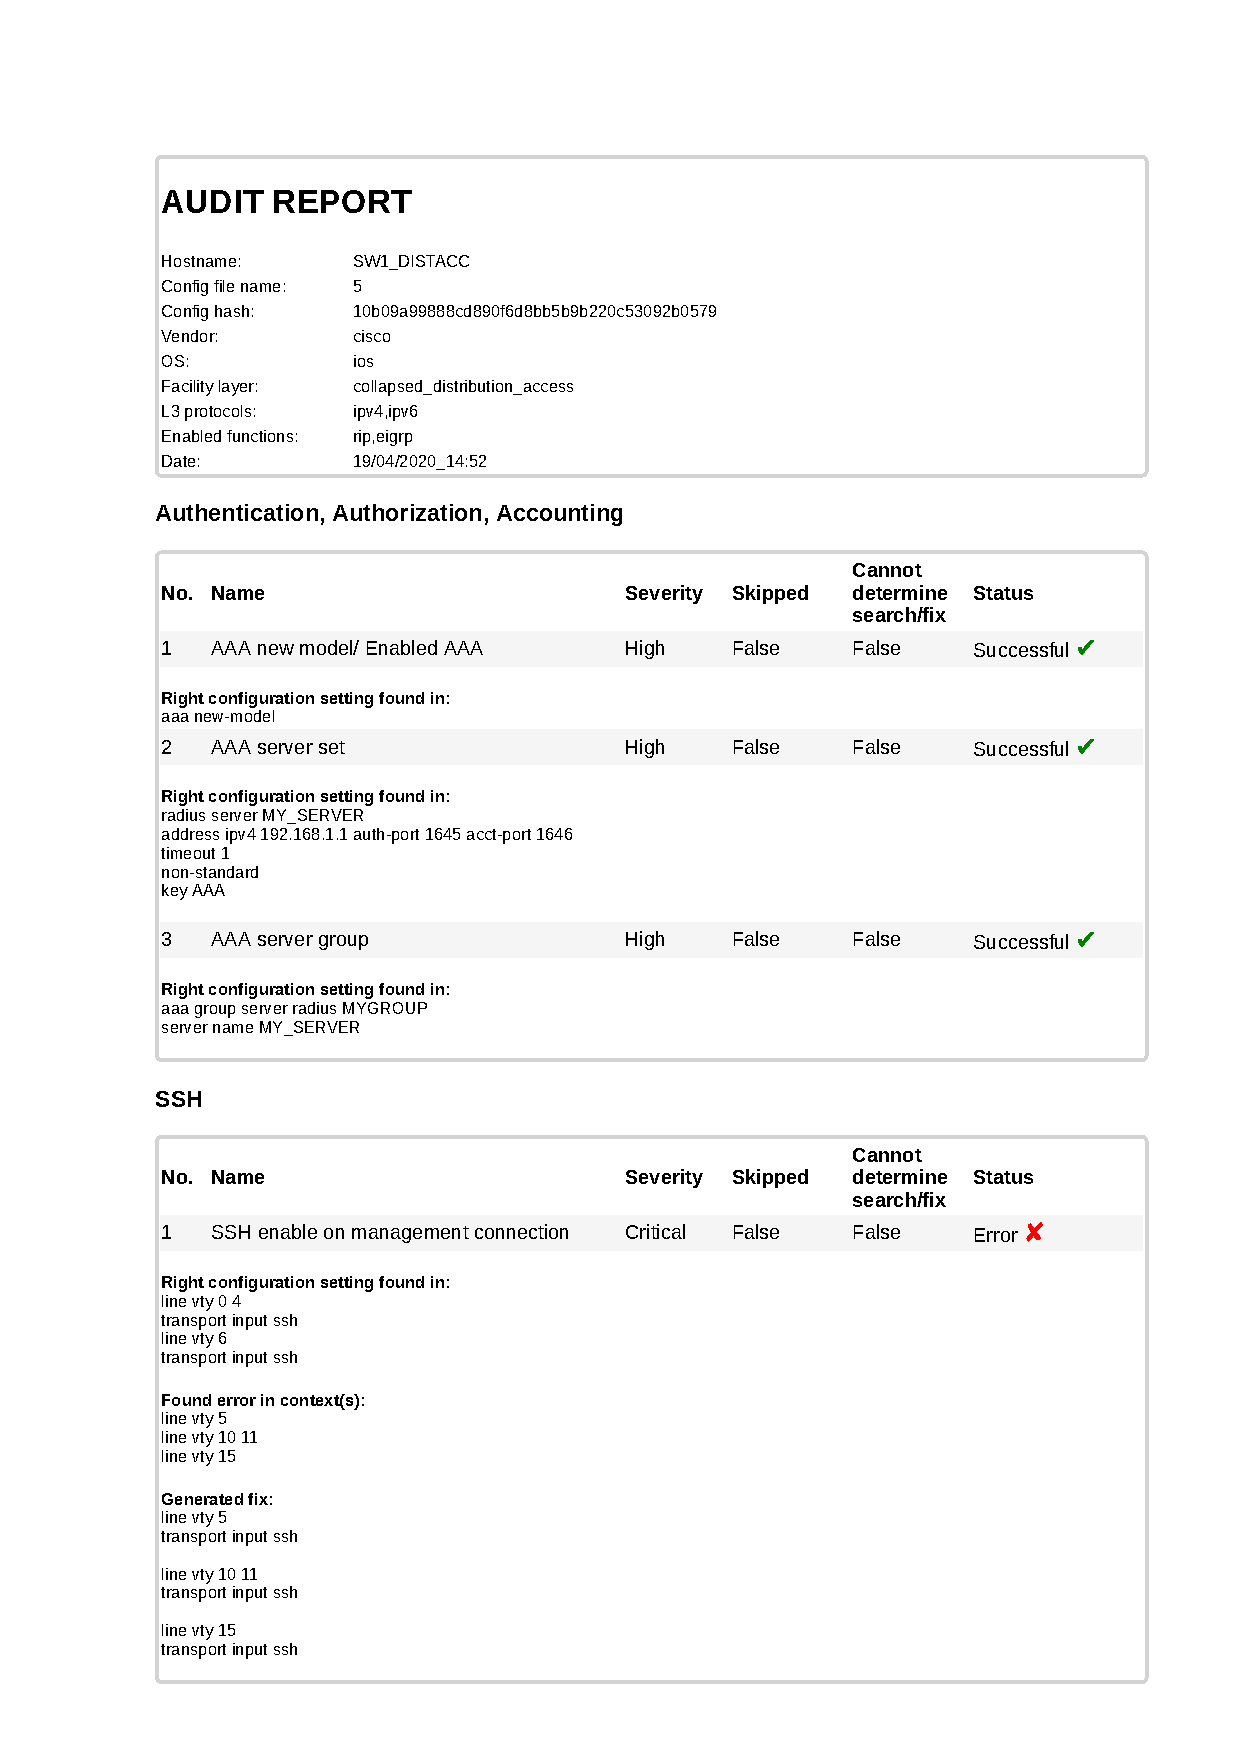
\includegraphics[scale=0.85]{obrazky/report_html_page_1.pdf}
	\end{center}
	
	\label{report_1}
\end{figure}
\begin{figure}[H]
	\begin{center}
		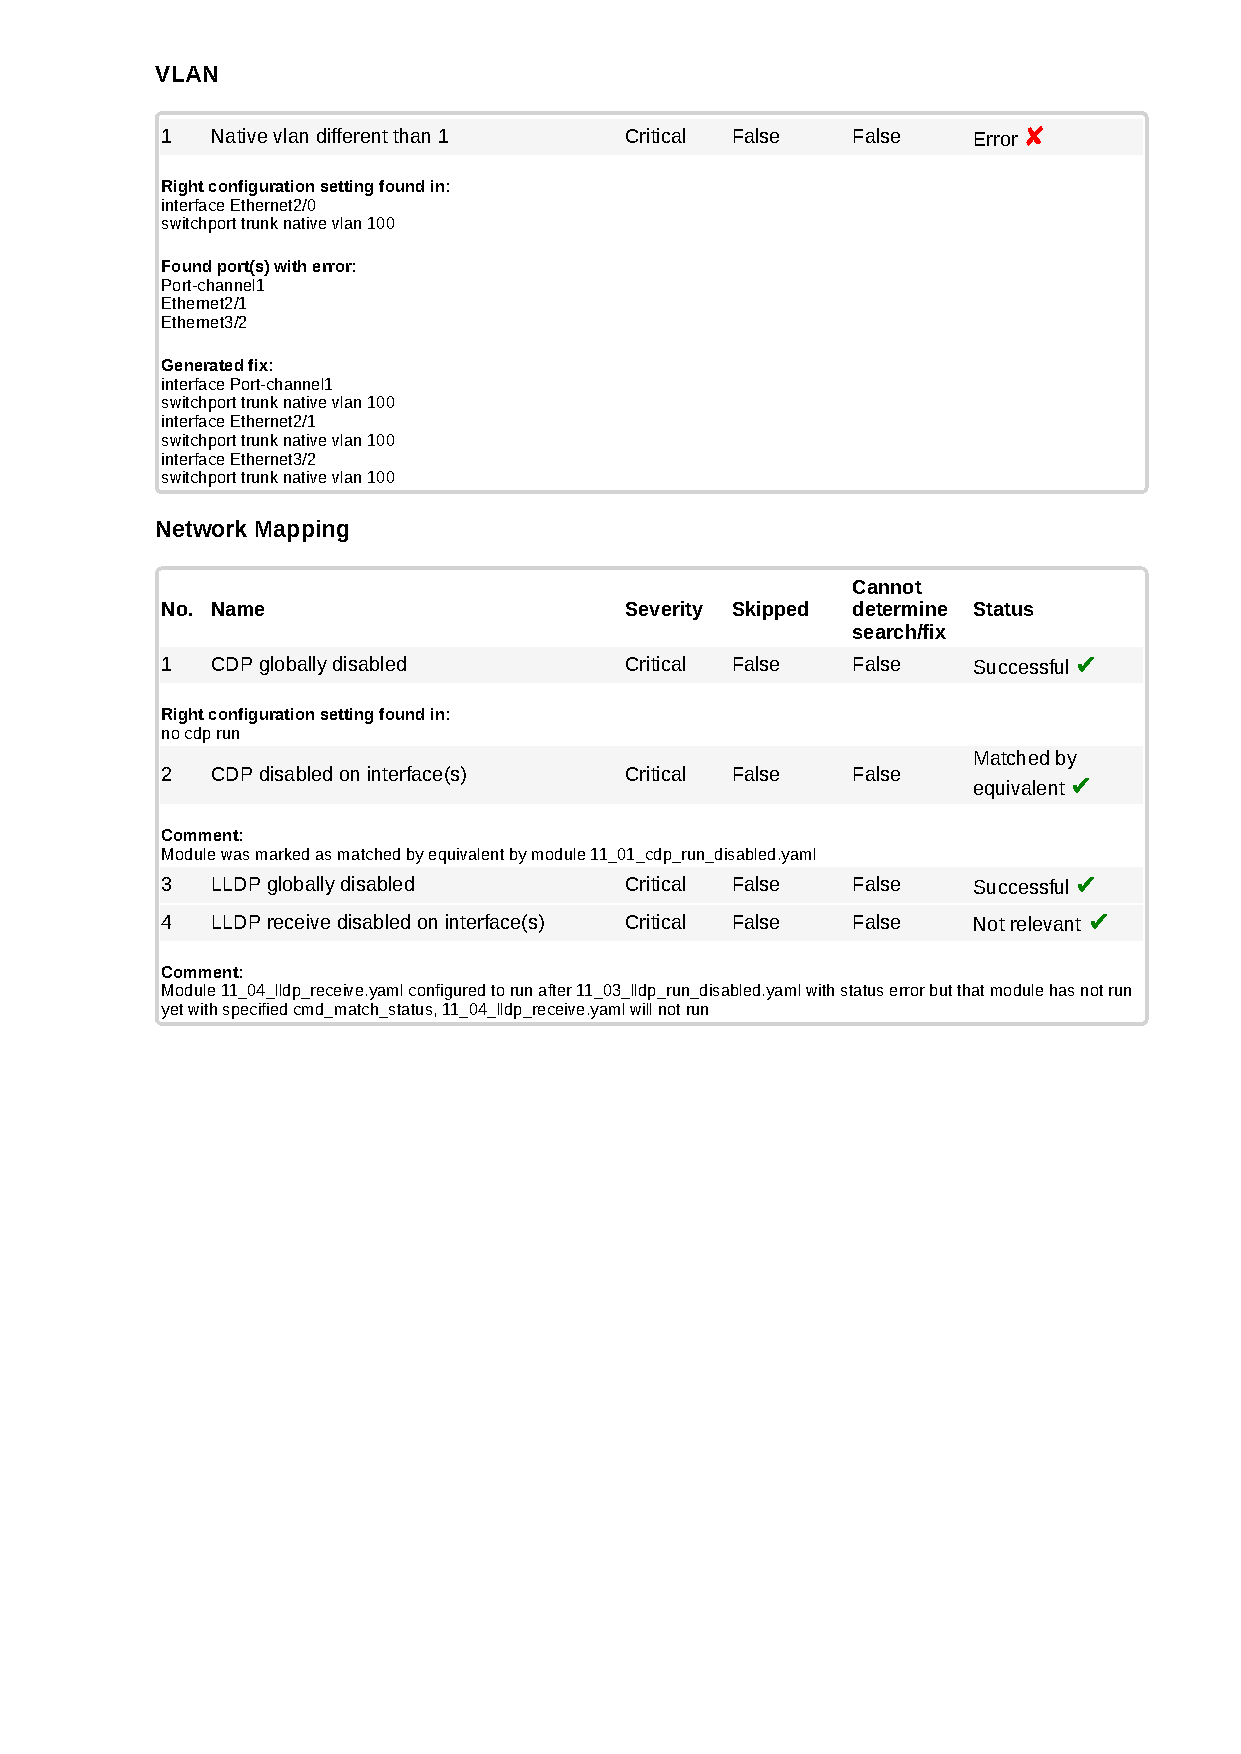
\includegraphics[scale=0.85]{obrazky/report_html_page_2.pdf}
	\end{center}
	
	\label{report_2}
\end{figure}

\section{Požiadavky programu}
Na bezproblémovú prácu s programom sú potrebné tieto náležitosti:
\begin{enumerate}
	\item Python 3.7.3 alebo vyšší
	\item Python modul \texttt{ruamel.yaml}
	\item Python modul \texttt{pdfkit} (voliteľný)\,--\,pri nenainštalovaní nebudú vygenerované PDF správy, ale iba HTML správy.
	\item Program \texttt{wkhtmltopdf} (voliteľný)\,--\,pri nenainštalovaní nebudú vygenerované PDF správy, ale iba HTML správy.
\end{enumerate}





